% [原文 p.175]
% 承接 p.174 末句（跨块句）。按 TIMELINE 规则，起于 p.174 的句子“……”由 appC1 写完；本块从“この要素 $c_p$ は”起译。
这个元素 $c_p$ 由
\[
  c_p=\gamma_p(1)=\mu^*(b^{p,1}),\qquad 1\in KR(S^{p,0})
\]
给出。

对任意 $Y$，射影 $X\times Y\to X$ 给出 KR 以及以 $Y$ 为系数的 KR 的完全系数序列。当 $Y$ 是球面时，得到下列这类 Gysin 序列中的一种。

\begin{proposition*}{C.3.2}
  射影 $\pi\colon S^{p,0}\to \mathrm{pt}$ 诱导出下列正合列。
  \[
    \cdots\to KR^{p-q}(X)\xrightarrow{\chi} KR^{-q}(X)
    \xrightarrow{\pi^*} KR^{-q}(X\times S^{p,0})
    \xrightarrow{\delta}\cdots
  \]
  其中 $\chi$ 是与 $(-\eta)^p$ 的乘法，$\eta\in KR^{-1}(\mathrm{pt})\cong\widetilde{KR}\bigl(P(\R^2)\bigr)$ 是约化实 Hopf 丛。
\end{proposition*}

\begin{proof}
  把 $\pi$ 换成与它等价的包含映射 $S^{p,0}\to B^{p,0}$。于是，空间对的 KR 群就是 $KR^{p,q}(X)$。为了计算 $\chi$，使用下面的交换图。
  \[
  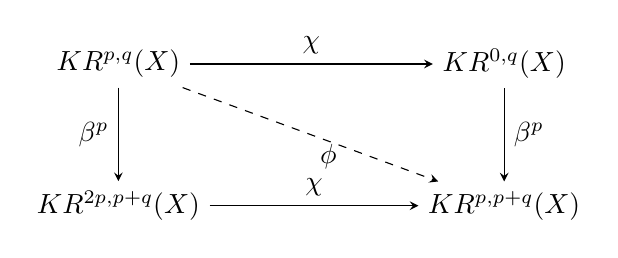
\begin{tikzpicture}[baseline=(current bounding box.center),>=stealth]
    \node (A) at (0,0) {$KR^{p,q}(X)$};
    \node (B) at (4.9,0) {$KR^{0,q}(X)$};
    \node (C) at (0,-1.8) {$KR^{2p,p+q}(X)$};
    \node (D) at (4.9,-1.8) {$KR^{p,p+q}(X)$};
    \draw[->] (A) -- node[above] {$\chi$} (B);
    \draw[->] (C) -- node[above] {$\chi$} (D);
    \draw[->] (A) -- node[left] {$\beta^p$} (C);
    \draw[->] (B) -- node[right] {$\beta^p$} (D);
    \draw[->,dashed] (A) -- node[below right] {$\phi$} (D);
  \end{tikzpicture}
  \]
  设 $\theta$ 为交换两个 $\R^{p,0}$ 所得到的 $KR^{2p,p+q}(X)$ 的自同构映射。此时，合成 $\chi\theta\beta^p$ 是乘以 $b^p$ 在
  % [原文 p.176]
  \[
    KR^{p,p}(*)\to KR^{0,p}(*)
  \]
  中的像的乘法。然而，这正是 $\eta^p$ 本身。剩下的只是计算 $\theta$。可是，照搬 [2, §2.4] 中给出的证明，即可证明 $\theta=(-1)^{p^2}=(-1)^p$。
\end{proof}

% [Tutor Note: 按 p.175 的图式，虚线对角 $\phi=\chi\theta\beta^p$ 是从 $KR^{p,q}(X)$ 到 $KR^{p,p+q}(X)$ 的复合；正文却写成 $KR^{p,p}(*)\to KR^{0,p}(*)$，把 $X$ 取成一点时下标 $p,q$ 如何对应，须按 C.3 的系数理论自行补足。又，此处的 $b^p$ 与 p.175 的 $c_p=\mu^*(b^{p,1})$ 中的 $b^{p,1}$ 关系原书未明说，此处照抄存疑。]

再详细考察命题 C.3.1 中的各个理论。当 $p=1$ 时，$S^{p,0}$ 就是共轭点对 $\{+1,-1\}$ 本身。$X\times\{+1,-1\}$ 上的实向量丛 $E$ 由它在 $X\times\{+1\}$ 上的限制——复向量丛 $E_+$——完全决定。因此得到下面的命题。

\begin{proposition*}{C.3.3}
  自然同构映射
  \[
    KR(X\times S^{1,0})\cong K(X)
  \]
  存在。
\end{proposition*}

特别要注意，它只依赖于 $X$ 的底层空间，而不依赖于 $X$ 的实结构。命题 C.3.1 给出的周期 2 确实与 $K(X)$ 的周期一致。进一步，命题 C.3.2 的正合列成为下面的样子。
\begin{equation}
  \cdots\to KR^{1-q}(X)\xrightarrow{\chi} KR^{-q}(X)
  \xrightarrow{\pi^*} K^{-q}(X)\xrightarrow{\delta} KR^{2-q}(X)\to\cdots \tag{C.3.4}
\end{equation}
其中 $\chi$ 是与 $-\eta$ 的乘法，$\pi^*=c$ 是复化。$\delta$ 的确定作为习题留给读者。（当 $X$ 上的对合为平凡时）这个正合列是众所周知的，但它一直是从正交群的周期性定理导出的。这里的步骤与此不同，反过来也可以用 (C.3.4) 证明正交群的周期性。作为替代，后面将从命题 C.3.1 的 $p=4$ 的情形更简单地导出这个正合列。

其次考虑命题 C.3.1 的 $p=2$ 的情形。此时，$KR^{-q}(X\times S^{2,0})$ 以 4 为周期。把它与自共轭理论 $KSC$ 等同起来。若 $X$ 是以 $\tau$ 为对合的实空间，则 $X$ 上的自共轭丛是指复向量丛 $E$ 与同构映射 $\alpha\colon E\to\tau^*(E)$ 的组 $(E,\alpha)$。这里考虑空间 $X\times S^{2,0}$，把 $S^{2,0}$ 分解为交为 $\{\pm 1\}$ 的两个半球面 $S^{2,0}_+$ 与 $S^{2,0}_-$。

% [原文 p.177]
\[
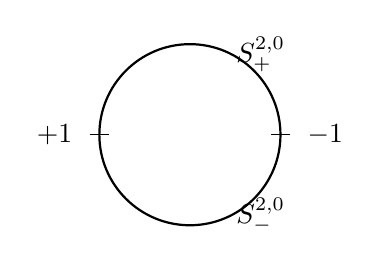
\begin{tikzpicture}[baseline=(current bounding box.center),scale=1]
  \draw[thick] (0,0) circle (1.15);
  \draw (-1.15,0) ++(-0.12,0) -- ++(0.24,0);
  \draw (1.15,0) ++(-0.12,0) -- ++(0.24,0);
  \node[left] at (-1.37,0) {$+1$};
  \node[right] at (1.37,0) {$-1$};
  \node at (0.9,1.02) {$S^{2,0}_+$};
  \node at (0.9,-1.02) {$S^{2,0}_-$};
\end{tikzpicture}
\]
显然，给定 $X\times S^{2,0}$ 上的实向量丛 $F$，等价于给定 $X\times S^{2,0}_+$ 上的复向量丛 $F_+$（它是 $F$ 的限制）连同同构映射
\[
  \phi\colon F|_{X\times\{+1\}}\to\tau^*\bigl(\overline{F}|_{X\times\{-1\}}\bigr).
\]
然而，$X\times\{+1\}$ 是 $X\times S^{2,0}_+$ 的变形收缩，因此除同伦差异外得到唯一的同构映射
\[
  \theta\colon F_+|_{X\times\{-1\}}\to F_+|_{X\times\{+1\}}
\]
（参见 [3, 引理 2.3]）。从而，给出 $\phi$ 等价于（除同伦差异外）给出同构映射
\[
  \alpha\colon E\to\tau^*(\overline{E})
\]
等价。其中 $E$ 是 $X$ 上的向量丛，映射 $x\mapsto(x,1)$ 与
\[
  \alpha_x=\theta_{(x,-1)}\phi_{(x,1)}
\]
由 $F_+$ 诱导而来。换言之，$X\times S^{2,0}$ 上实向量丛的同构类与 $X$ 上自共轭丛的同伦类一一对应。而且，这个对应显然与张量积相容。现在，用 $KSC(X)$ 表示 $X$ 上自共轭丛的同伦类的 Grothendieck 群。当 $\tau$ 平凡时，这个 Grothendieck 群与 [1] 及 [7] 的定义一致。此时，下面的命题成立。

% [Tutor Note: 这一步是本节的关键：$X\times S^{2,0}_+$ 上的复丛 $F_+$ 配上 $\theta$，就等价于给 $X$ 上的丛 $E$ 一个与对合 $\tau$ 相容的同构 $\alpha\colon E\to\tau^*(\overline{E})$。注意 $\alpha$ 的反线性来自复共轭，而 $\theta$ 的同伦类才是唯一被记住的不变量，所以“实丛的同构类”与“自共轭丛的同伦类”才一一对应。]

\begin{proposition*}{C.3.5}
  存在下列环的自然同构映射。
  % [原文 p.178]
  \[
    KSC(X)\to KR(X\times S^{2,0}).
  \]
\end{proposition*}

把命题 C.3.2 的正合列中令 $p=2$，得到正合列
\begin{equation}
  \cdots\to KR^{2-q}(X)\xrightarrow{\chi} KR^{-q}(X)
  \xrightarrow{\pi^*} KSC^{-q}(X)\xrightarrow{\delta} KR^{3-q}(X)\to\cdots \tag{C.3.6}
\end{equation}
其中 $\chi$ 是与 $\eta^2$ 的乘法，$\pi^*$ 是把任意实向量丛（令 $\alpha=\tau$）对应到与它相伴的自共轭丛的映射。KSC 中的周期性由乘以 $KSC^{-4}(*)$ 的生成元给出。

最后考察 $p=4$ 的情形。为此需要下面的引理。

\begin{lemma*}{C.3.7}
  设 $\eta\in KR^{-1}(*)$ 为 C.2 节定义的元。此时 $\eta^3=0$。
\end{lemma*}

\begin{proof}
  这可以用线性代数证明。事实上，回想存在同态映射 $\alpha\colon A_k\to KR^{-k}(*)$（[4, §11]）。其中 $A_k$ 是用 Clifford 代数定义得到的群。此时，$\eta$ 是 $A_1\cong\Z/2$ 的生成元的像，而 $A_3=0$。同态映射 $\alpha_k$ 是乘性的（[4, §11.4]），故可知 $\eta^3=0$。
\end{proof}

\begin{corollary*}{C.3.8}
  对任意 $p\ge 3$，存在下列短正合列。
  \[
    0\to KR^{-q}(X)\xrightarrow{\pi^*} KR^{-q}(X\times S^{p,0})
    \xrightarrow{\delta} KR^{p+1-q}(X)\to 0
  \]
\end{corollary*}

\begin{proof}
  这由引理 C.3.7 与命题 C.3.2 导出。
\end{proof}

按照命题 C.3.1 之后的注，$KR(X\times S^{4,0})$ 的周期性由乘以下列元素给出：
\[
  c_4=\mu_4^*(b^{4,1})\in KR^{-8}(S^{4,0}).
\]
现在，回想 $A_8\cong\Z$，并且 $A_8$ 由（作为 Clifford 代数 $C_8$ 的不可约分次模的代表元的）元素 $\lambda$ 生成（[4, Table 2]）。同态映射

% [原文 p.179]
\[
  \alpha\colon A_8\to KR^{-8}(*)
\]
由此得到元素 $\alpha(\lambda)\in KR^{-8}(*)$。于是，$c_4$ 与 $\alpha(\lambda)$ 之间的关系由下面的引理给出。

\begin{lemma*}{C.3.9}
  用 $1$ 表示 $KR(S^{4,0})$ 的单位元。此时，下列等式成立。
  \[
    c_4=\alpha(\lambda)\cdot 1\in KR^{-8}(S^{4,0}).
  \]
\end{lemma*}

引理 C.3.9 的证明需要详细考察 Clifford 代数，故推迟到更详细讨论 Clifford 代数的 C.4 节。

利用引理 C.3.9，证明下面定理的准备已经就绪。

\begin{theorem*}{C.3.10}
  设 $\lambda\in A_8$，$\alpha(\lambda)\in KR^{-8}(*)$ 如前所述。此时，乘以 $\alpha(\lambda)$ 诱导出下列同构映射。
  \[
    KR(X)\to KR^{-8}(X).
  \]
\end{theorem*}

\begin{proof}
  在系 C.3.8 的正合列上乘 $\alpha(\lambda)$，得到下列正合列的交换图。
  \[
  \begin{array}{ccccccccc}
    0 & \to & KR^{-q}(X) & \to & KR^{-q}(X\times S^{4,0}) & \to & KR^{5-q}(X) & \to & 0\\[1mm]
      &     & \downarrow_{\phi_q} & & \downarrow_{\psi_q} & & \downarrow_{\phi_{5-q}} & & \\[1mm]
    0 & \to & KR^{-q-8}(X) & \to & KR^{-q-8}(X\times S^{4,0}) & \to & KR^{-3-q}(X) & \to & 0
  \end{array}
  \]
  由引理 C.3.9，可知 $\psi_q$ 与周期性定理的同构映射 $\gamma_4$ 一致。因此，$\phi_q$ 对所有 $q$ 都是单射。上面图式中 $\phi_{5-q}$ 是单射，再结合 $\psi_q$ 是同构映射这一事实，便可导出 $\phi_q$ 是满射。因此，$\phi_q$ 是同构映射。
\end{proof}

\para{注.}
若 $X$ 上的对合为平凡，则 $KR(X)=KO(X)$，定理 C.3.10 就是通常的“实周期性定理”。

% [原文 p.180]
考察各种包含映射 $S^{q,0}\to S^{p,0}$，可以得到有趣的正合列。为了考虑空间对，需要下面的引理。

\begin{lemma*}{C.3.11}
  带基点的实空间 $S^{p,0}/S^{q,0}$ 与
  \[
    (S^{p-q,0}\times B^{q,0})/(S^{p-q,0}\times S^{q,0})
  \]
  同构。
\end{lemma*}

\begin{proof}
  $S^{p,0}-S^{q,0}$ 与 $S^{p-q,0}\times\R^{q,0}$ 同胚。把它紧化即可。
\end{proof}

\begin{corollary*}{C.3.12}
  自然同构映射
  \[
    KR(X\times S^{p,0},X\times S^{q,0})\cong KR^{0,q}(X\times S^{p-q,0})
  \]
  存在。
\end{corollary*}

考虑到系 C.3.8，有趣的只是 $p,q$ 取小值的情形，特别是 $p=2$、$q=1$ 的情形重要。此时得到下列正合列（参见 [1]）。
\[
  \cdots\to K^{-1}(X)\to KSC(X)\to K(X)\to K(X)\to\cdots
\]
事实上，系 C.3.8 的正合列（对 $p\ge 3$）
\begin{equation}
  KR^{-q}(X\times S^{p,0})\cong KR^{-q}(X)\oplus KR^{p+1-q}(X) \tag{C.3.13}
\end{equation}
自然地分裂。为证明这一点，只需考虑 $p=3$ 的情形。因为一般情形可由限制得到的下列交换图（$p\ge 4$）导出。
\[
\begin{array}{ccc}
  0\to KR(X) & \to & KR(X\times S^{p,0})\\[1mm]
  \big\downarrow & & \big\downarrow\\[1mm]
  0\to KR(X) & \to & KR(X\times S^{3,0})
\end{array}
\]
这里，$S^{3,0}$ 是以对跖映射为对合的 2 维球面，可以看作 $P(\C^3)$ 中由 $\sum_{i=0}^2 z_i^2=0$ 给出的二次曲面。

% [Tutor Note: 系 C.3.8 的正合列 $0\to KR^{-q}(X)\to KR^{-q}(X\times S^{p,0})\to KR^{p+1-q}(X)\to 0$ 在 $p\ge3$ 时分裂，本质原因是 $\eta^3=0$（引理 C.3.7）：正合列由乘以 $\eta^p$ 给出，而 $\eta^3=0$ 使得再乘一次就消失。$p=3$ 的情形用 $S^{3,0}\subset P(\C^3)$ 的二次曲面结构及 C.5 节的左逆命题处理。]

% [原文 p.181]
按 C.5 节不加证明地叙述的命题，当 $Y$ 是二次曲面时，可知
\[
  KR(X)\to KR(X\times Y)
\]
有标准的左逆映射。这样就证明了 (C.3.13)。

\section{与 Clifford 代数的关系}

\takeaway{本节把分次实 $\operatorname{Cliff}(\R^{p,q})$ 模的 Grothendieck 群与 $KR$ 联系起来：以限制映射的余核定义 $A(p,q)$，得到乘性同态 $\alpha\colon A(p,q)\to KR^{p,q}(*)$，并用外代数 $\Lambda^*(\C^1)$、$\Lambda^*(\C^4)$ 造出 $A_8$ 的生成元 $\lambda$，为证明 $c_4=\alpha(\lambda)\cdot1$ 作准备。}

用 $\operatorname{Cliff}(\R^{p,q})$ 表示 $\R^{p,q}$ 上由二次曲面
\[
  -\Bigl(\sum_{i=1}^p y_i^2+\sum_{j=1}^q x_j^2\Bigr)
\]
定义的（$\R$ 上的）Clifford 代数。$\R^{p,q}$ 的对合 $(y,x)\mapsto(-y,x)$ 诱导 $\operatorname{Cliff}(\R^{p,q})$ 的对合自同构 $a\mapsto\bar a$\footnote{这个记号与 [4, §1] 的记号不同。在 [4, §1] 中（对 $q=0$）这个记号称作 $\alpha$，而上划线用于反自同构映射。}。

设 $M=M^0\oplus M^1$ 为 $\Z/2$ 分次复 $\operatorname{Cliff}(\R^{p,q})$ 模。当 $M$ 具有满足下列条件的实结构（即反线性对合 $m\mapsto\bar m$）时，称 $M$ 为 $\Z/2$ 分次实 $\operatorname{Cliff}(\R^{p,q})$ 模。
\begin{enumerate}[label=(\roman*),leftmargin=2.2em,itemsep=2pt]
  \item $\Z/2$ 分次与实结构相容，即
  \[
    \overline{M^i}=M^i\qquad(i=0,1)
  \]
  成立。
  \item 对 $a\in\operatorname{Cliff}(\R^{p,q})$ 及 $m\in M$，有 $\overline{am}=\bar a\,\bar m$。
\end{enumerate}
当 $p=0$ 时——从而 $\operatorname{Cliff}(\R^{p,q})$ 上的对合为平凡时——
\[
  M_\R=M^0_\R\oplus M^1_\R=\{m\in M\mid \bar m=m\}
\]
是通常意义下的 $\Z/2$ 分次实模（[4] 的记法中为 $C_q$ 模），注意这一点。

[4] 的基本构造法对这个新情形也适用。因此，分次实 $\operatorname{Cliff}(\R^{p,q})$ 模 $M=M^0\oplus M^1$ 确定三元组 $(M^0,M^1,\sigma)$。

% [原文 p.182]
其中 $\sigma\colon S^{p,q}\times M^0\to S^{p,q}\times M^1$ 是由
\[
  \sigma(s,m)=(s,sm)
\]
给出的实同构映射。这样便得到同态映射
\[
  h\colon M(p,q)\to KR^{p,q}(*),
\]
其中 $M(p,q)$ 是分次实 $\operatorname{Cliff}(\R^{p,q})$ 模的 Grothendieck 群。若 $M$ 是 $\operatorname{Cliff}(\R^{p,q+1})$ 模的限制，则 $\sigma$ 可延拓到 $S^{p,q+1}$ 上。（用 $S^{p,q+1}_+$ 表示关于最后坐标的上半球面时，）射影
\[
  S^{p,q+1}_+\to B^{p,q}
\]
是实空间的同构映射，故可知 $M$ 定义 $KR^{p,q}(*)$ 的零元。因此，把限制映射
\[
  M(p,q+1)\to M(p,q)
\]
的余核定义为 $A(p,q)$，则可知 $h$ 诱导同态映射
\[
  \alpha\colon A(p,q)\to KR^{p,q}(*).
\]
进一步，如 [4] 所述，$\alpha$ 是乘性的。注意对 $p=0$，这个 $\alpha$ 与 [4] 中定义的本质上相同。因为
\[
  A(0,q)\cong A_q,\qquad KR^{0,q}(*)\cong KO^{-q}(*)
\]
成立。外代数 $\Lambda^*(\C^1)$ 由
\[
  z(1)=ze,\qquad z(e)=-\bar z 1
\]
自然成为 $\operatorname{Cliff}(\R^{1,1})$ 模。其中 $1\in\Lambda^0(\C^1)$ 与 $e\in\Lambda^1(\C^1)$ 是标准生成元。用 $\lambda_1\in A(1,1)$ 表示由这个模 $\Lambda^*(\C^1)$ 定义的元。考虑 $b\in KR^{1,1}(*)$ 的定义，则

% [原文 p.183]
\[
  \alpha(\lambda_1)=-b
\]
而 $\alpha$ 是乘性的，故
\[
  \alpha(\lambda_1^4)=b^4.
\]
设 $M$ 为分次 $\operatorname{Cliff}(\R^{4,4})$ 模（与 [4, §11] 同样，$M$ 可由外代数 $\Lambda^*(\C^4)$ 构成）。又，设 $e_1,e_2,e_3,e_4$ 为 $\R^{4,0}$ 的标准基，令 $w=e_1e_2e_3e_4\in\operatorname{Cliff}(\R^{4,4})$。此时
\[
  w^2=1,\qquad \bar w=w,\qquad wz=\bar z w\quad(z\in\C^4=\R^{4,4})
\]
成立。因此，若用
\[
  \tilde m=-w\bar m
\]
定义 $M$ 上新的反线性对合 $m\mapsto\tilde m$，则
\begin{align*}
  \widetilde{zm} &= -w\overline{zm} = -w\bar z\bar m = -zw\bar m\\
  &= z\tilde m
\end{align*}
成立。于是，$M$ 由这个新的对合（或实结构）成为分次实 $\operatorname{Cliff}(\R^{0,8})$ 模。这在 [4] 的记法中是 $C_8$ 模。把这个分次实 $\operatorname{Cliff}(\R^{0,8})$ 模记作 $N$。考虑维数（参见 [4, Table 2]），$N$ 必须是两个不可约 $C_8$ 模之一。但是，复化（即忽略对合）后得到与 $M$ 相同的东西，所以 $N$ 是 [4] 中写作 $\lambda$ 的 $A_8$ 的元。

% [Tutor Note: 新对合 $\tilde m=-w\bar m$ 的要点是 $w^2=1$、$\bar w=w$ 且 $wz=\bar zw$（$w\in\operatorname{Cliff}(\R^{4,4})$ 为体积元）。这三条正好使 $z\tilde m=\widetilde{zm}$，即新对合与 $\C^4=\R^{4,4}$ 的模结构相容；符号取负是为了让 $\bar{\tilde m}=m$（对合性）。$\Lambda^*(\C^4)$ 在旧结构下是 $C_4$ 模、在新结构下是 $C_8$ 模，这正是维数 4 与 8 的跳跃所在。]

到此为止的准备使我们能够进入引理 C.3.9 的证明。要证明的是：在映射
\[
  \mu_4\colon S^{4,0}\times\R^8\to S^{4,0}\times\C^4
\]
之下，由 $M$ 定义的 $KR^{4,4}(S^{4,0})$ 的元素提升为由 $N$ 定义的 $KR^{-8}(S^{4,0})$ 的元素。为证明这一点，只需证明实同构映射的图式

% [原文 p.184]
\begin{equation}
  \begin{array}{ccc}
    S^{4,0}\times\R^8\times N & \xrightarrow{\ \nu\ } & S^{4,0}\times\C^4\times M\\[2mm]
    \downarrow & & \downarrow\\[2mm]
    S^{4,0}\times\R^8\times N & \xrightarrow{\ \nu\ } & S^{4,0}\times\C^4\times M
  \end{array} \tag{C.4.1}
\end{equation}
可交换。其中 $\nu$ 与 $\mu_4$ 相容（即对某个 $m$，$\nu(s,x,y,n)=(s,x+isy,m)$），纵向箭头由模结构（即 $(s,x,y,n)\mapsto(s,x,y,(x,y)n)$）给出。

现在，考虑代数 $\operatorname{Cliff}(\R^{4,0})=C_4$。偶数次部分 $C_4^0$ 与 $\HH\oplus\HH$ 同构（[4, Table 1]）。进一步，它的中心由 $1$ 与 $w=e_1e_2e_3e_4$ 生成，两个投影是 $\frac12(1\pm w)$。更具体地，把嵌入
\[
  \xi\colon \HH\to\operatorname{Cliff}^0(\R^{4,0})
\]
定义为
\[
  \xi(1)=\frac{1+w}{2},\quad
  \xi(i)=\frac{1+w}{2}e_1e_2,\quad
  \xi(j)=\frac{1+w}{2}e_1e_3,\quad
  \xi(k)=\frac{1+w}{2}e_1e_4.
\]
于是，嵌入
\[
  \eta\colon S(\HH)\to\operatorname{Spin}(4)\subset\Gamma_4
\]
可以由 $\eta(s)=\xi(s)+\frac12(1-w)$ 定义。其中 $\Gamma_4$ 是 Clifford 群（[4, 定义 3.1]），$S(\HH)$ 表示范数为 1 的四元数。同态映射的合成
\[
  S(\HH)\to\operatorname{Spin}(4)\to\operatorname{SO}(4)
\]
与由 $S(\HH)$ 左乘给出的对 $\R^4=\HH$ 的自然作用\footnote{把 $1,i,j,k$ 依次与标准基 $e_1,e_2,e_3,e_4$ 等同。}一致，这一点也容易验证。

% CHUNK appC2 DONE

